\chapter{Software Defined Radio}
\label{chap:sdr}

\section{Overview}%ok
\label{sdr:overview}

In the modern world everything is becoming \"smarter\", and the cloud paradigm is
creating a new way to organize the infrastructure, so telecommunications will
also be affected by such changes. The RAN as a service  paradigm and cloud
requires devices which are both scalable and reconfigurable following customer
demands, in order to accomplish that there is a lot of schemes and theories
involved, but this work will focus on a device that fits in the \emph{Software
Defined Radio} scope, which is defined according to the \emph{SDR Forum}
\cite{web:sdrforum} as:

say{radios that provide software control of a variety of modulation techniques,
wide-band or narrow-band operation, communications security functions (such as
hopping), and waveform requirements of current \& evolving standards over a
broad frequency range.}

In short, Software-Defined Radio (SDR) refers to the technology wherein software
modules running on a generic hardware platform consisting of DSPs, FPGA and
general purpose microprocessors are used to implement radio functions such as
generation of transmitted signal (modulation) at transmitter and
tuning/detection of received radio signal (demodulation) at receiver.\\

This is a very powerful concept and it has been idealized over 20 years ago,
however only with the recent era , after 2000, DSP and FPGA technology grew and
its implementation became feasible \cite{ladimer2009}. SDR has some very
interesting applications, in this chapter the educational and telecommunications
applications of SDR shall be explored.\\

For its elastic characteristic, SDR is recommended or not depending on the
application because it is more costly than a normal analog radio, thus
\emph{what is the real advantage in SDR?}, according to worldwide
telecommunication reports and works, every time a standard is changed there is a
huge cost in equipment change in both user and provider so SDR tries to reduce
these costs by maintaining legacy systems while being able to upgrade to newer
systems\cite{dayananda2012}.\\

This fact generated a lot of interest in the wireless communication industry
because of the economic advantages SDR could bring. Another great advantage for
companies to implement SDR is that they can use the same hardware and such
hardware would work in all communication schemes around the world. The use of
SDR is growing in the industry and seems to be a promise for the Cloud-RAN
environment, where radio infrastructure would adapt itself to the customer
needs.

\section{Cloud Overview}
\label{sec:sdr_cloud}

Cloud computing is a computing paradigm, where a large variety of systems are
connected through networks, being able to provide dynamically scalable
infrastructure for application, data and file storage. With the advent of this
technology, the cost of computation resources, application hosting, content
storage and delivery is reduced significantly. \\

Cloud computing is a practical approach to experience direct cost benefits and
it has the potential to transform a data center from a capital-intensive set up
to a variable priced environment. \\

The idea of cloud computing is based on a very fundamental principle of
\emph{reusability of IT resources}. The difference that cloud computing brings
compared to traditional concepts of \"grid computing\", \"distributed computing\",
\"utility computing\", or \"autonomic computing\" is to broaden horizons across
organizational boundaries.\\

There are three main types of cloud in current use:

\begin{itemize}
    \item \textbf{Infrastructure as a Service (IaaS):} also referred to as
    Resource Clouds, provide (managed and scalable) resources as services to
    the user - in other words, they basically provide enhanced virtualization
    capabilities. Servers, storage systems, switches, routers, and other systems
    are pooled and made available to handle workloads that range from application
    components to high-performance computing applications. For 5G there is the
    idea to implement RAN as a Service or C-RAN, meaning that all the
    telecommunication devices can be used on an on-demand basis by costumers.

    \item \textbf{Platform as a Service (PaaS):} provide computational resources
    via a platform upon which applications and services can be developed and hosted.
    PaaS typically makes use of dedicated APIs to control the behavior of a server
    hosting engine which executes and replicates the execution according to user
    requests (e.g. access rate).

    \item \textbf{Software as a Service (IaaS):}Features a complete application
    offered as a service on demand. A single instance of the software runs on the
    cloud and services multiple end users or client organizations.
\end{itemize}

With the recent crisis in economic markets, companies goal changed from selling
devices to selling services, this does not mean that the company shall not
develop more devices, this means that they can fulfill costumers and operators
needs, for example, if a company needs a fiber optics backbone, the
telecommunications companies can sell the service, if they do not do so the
company can develop is own backbone as Google did with Google fiber, which is
bad for the operators and telecommunication companies.\\

\section{Gnuradio}
\label{sdr:gnuradio}

When SDR is mentioned the first thing that comes in mind is Gnuradio, because it
is a Open Source Software widely used in academic environment to teach and
research software defined Radios and implement very interesting applications.

\subsection{Gnuradio Project}

%inserir figura gnuradio
\begin{figure}[htbp]
    \centering
    
\includegraphics[width=0.65\textwidth]{./figures/gnuradio}
    \caption{ Gnuradio Logo
    \label{fig:gnuradiologo}}
\end{figure}

GNU Radio is a free \& open-source software development toolkit that provides
signal processing blocks to implement software radios. It can be used with
low-cost external RF hardware to implement software-defined radios, or without
hardware in a simulation environment. It is widely used in radio amateur,
academic and commercial environments to support both wireless communications
research and real-world radio systems.

\subsection{Capabilities}

GNU Radio performs all the signal processing. It is possible write applications
to receive data out of digital streams or to push data into digital streams,
which is then transmitted using hardware (USRP). GNU Radio has filters, channel
codes, synchronization elements, equalizers, demodulators, vocoders, decoders,
and many other elements , these elements are represented as blocks, which are
typically found in radio systems. It also includes a method of connecting these
blocks and then manages how data is passed from one block to another. Extending
GNU Radio is straightforward, because everything is modular, if there is need
for a block, it is just a matter of following the conventions and the block can
easily fit in the system.\\

Since GNU Radio is a software, it can only handle digital data. Usually, complex
baseband samples are the input data type for receivers and the output data type
for transmitters. Analog hardware is then used to shift the signal to the
desired center frequency. That requirement aside, any data type can be passed
from one block to another - be it bits, bytes, vectors, bursts or more complex
data types.\\

GNU Radio applications are primarily written using the Python programming
language, while the supplied, performance-critical signal processing path is
implemented in C++ using processor floating point extensions, where available.
Thus, the developer is able to implement real-time, high-throughput radio
systems in a simple-to-use, rapid-application-development environment. Gnuradio
also has a graphical interface where all the blocks are represented and it is
possible to assembly a system like a block diagram, this software is the
Gnuradio-companion\\

\subsection{USRP - Universal Software Radio Peripheral}

USRP stands for Universal Software Radio Peripheral and it is a hardware
developed by Ettus research, a National Instruments company. This hardware is
basically an FPGA and a transceiver connected allows the systems made inside the
Gnuradio software to be implemented in real-world, it means that USRP is a
hardware for implementing Software Radios, in the figure \ref{fig:usrpbd} it is
possible to see the basic components of a USRP.\\

%usrp n210 block diagram
\begin{figure}[htbp]
    \centering
    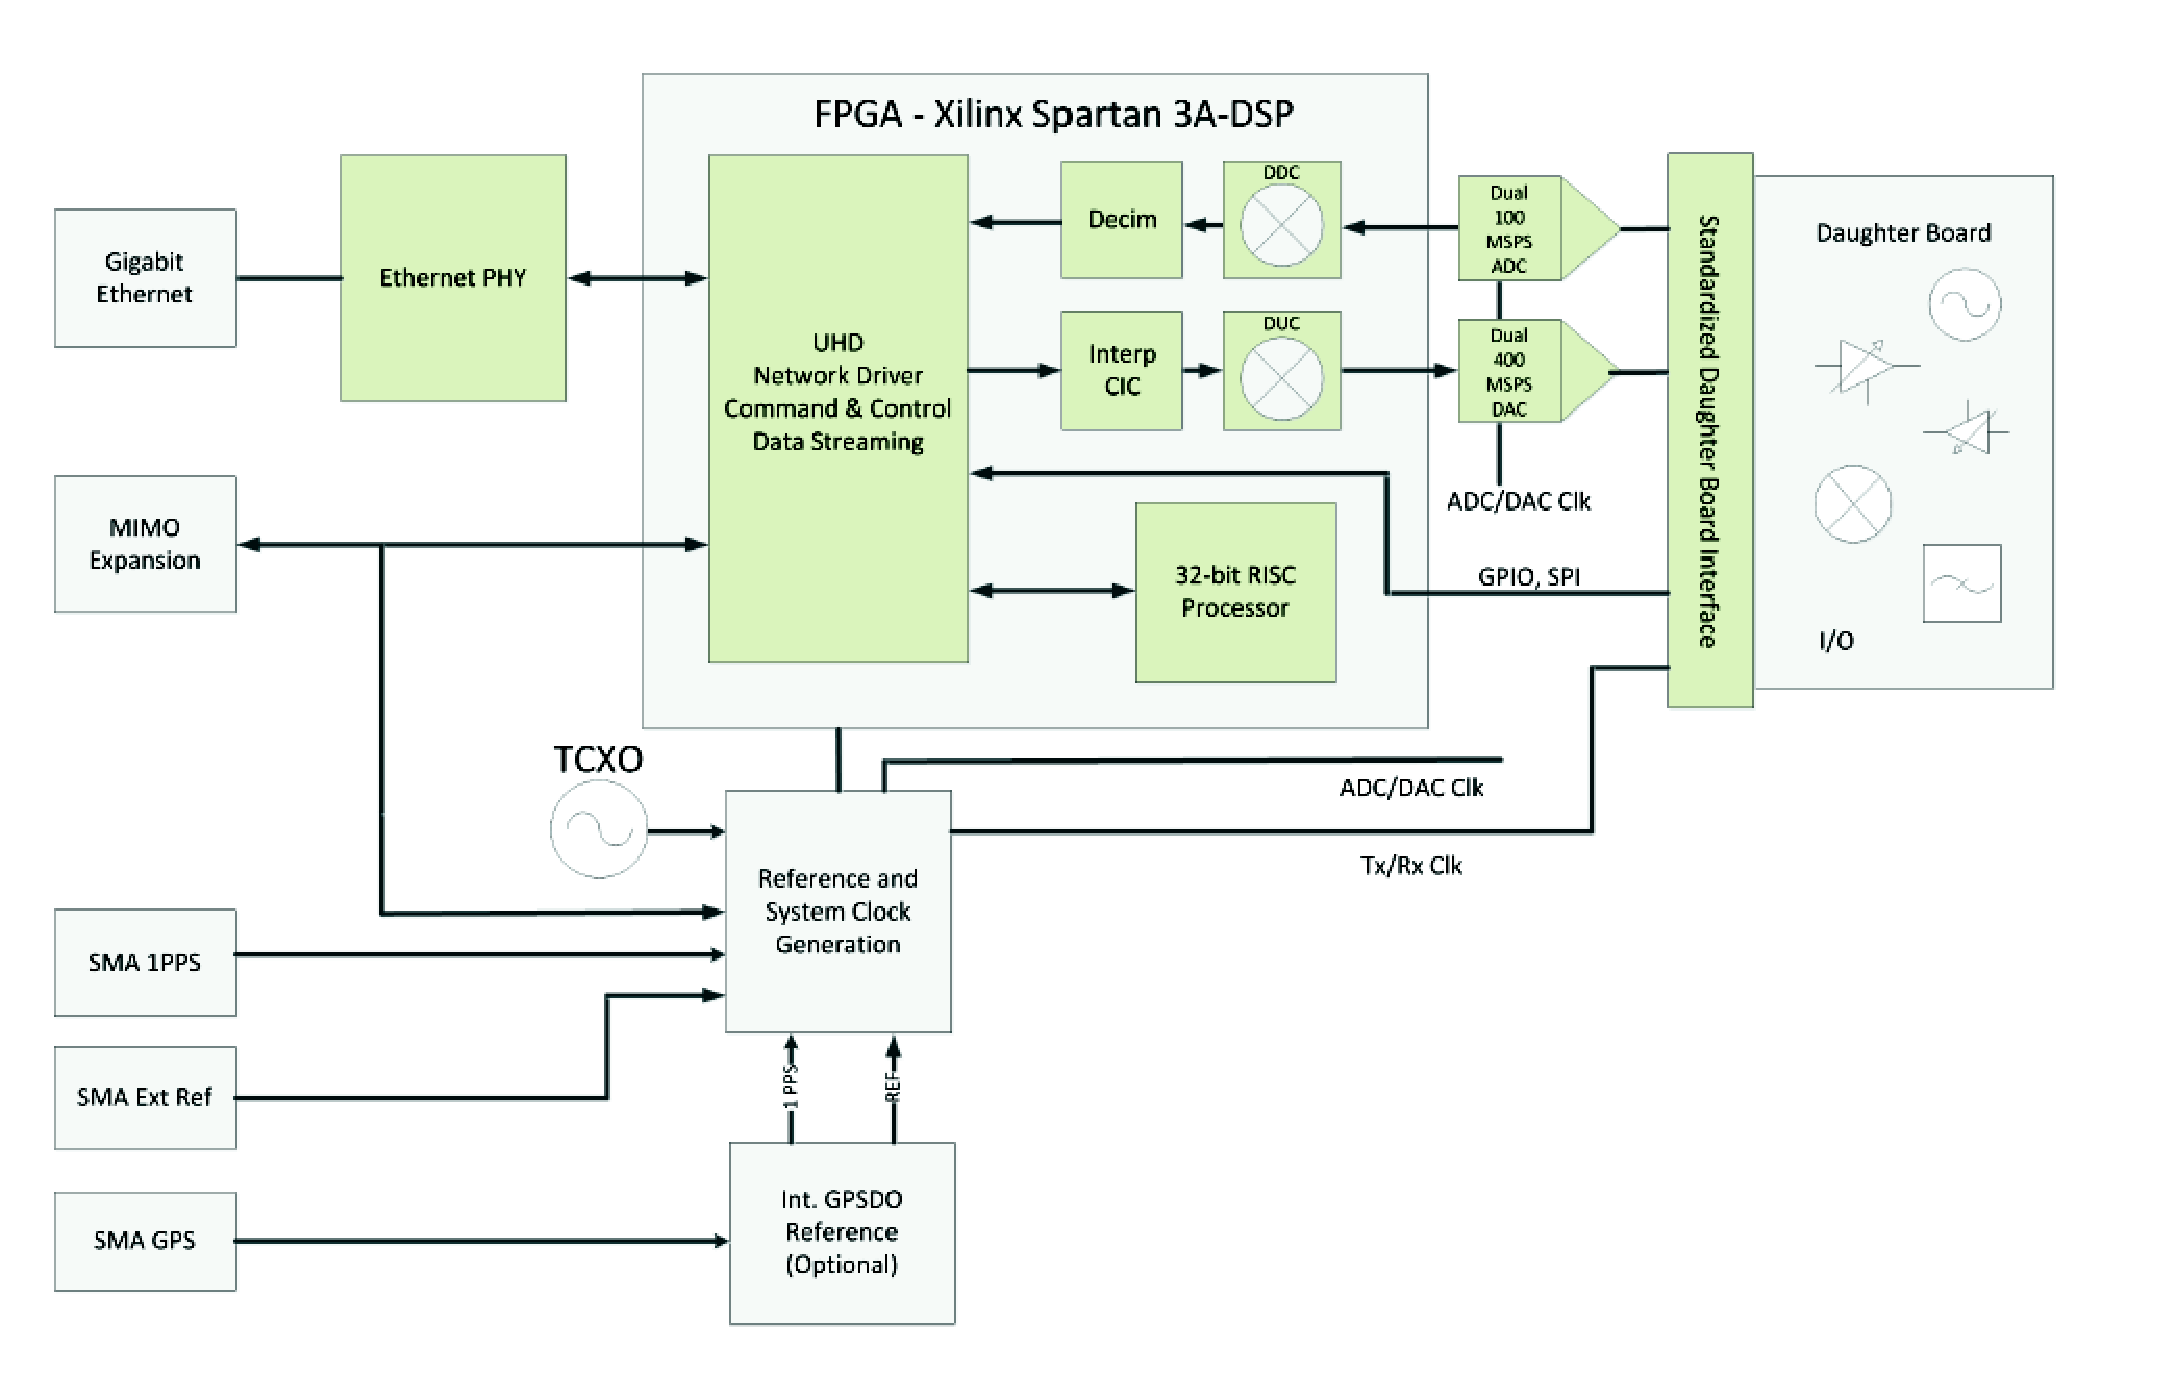
\includegraphics[width=0.65\textwidth]{./figures/usrp_bd}
    \caption{ USRP N2010 block diagram
    \label{fig:usrpbd}}
\end{figure}

The USRP communicates with the computer by the UHD (USRP Hardware Driver), and
gnuradio automatically recognizes it, making possible to send and receive
signals in the desired band. Gnuradio can read and write in the USRP from both
USB and ETHERNET connection, which makes easy to implement the gnuradio
generated digital systems in a real communication channel. USRP is not a
hardware exclusive to gnuradio, there are other communications engineering
softwares which are able to use USRP, like Matlab's simulink.\\

Below there is a frontal image of the USRP N210 in figure \ref{fig:usrp}, which
has Ethernet interface.\\


%figura usrp
\begin{figure}[htbp]
    \centering
    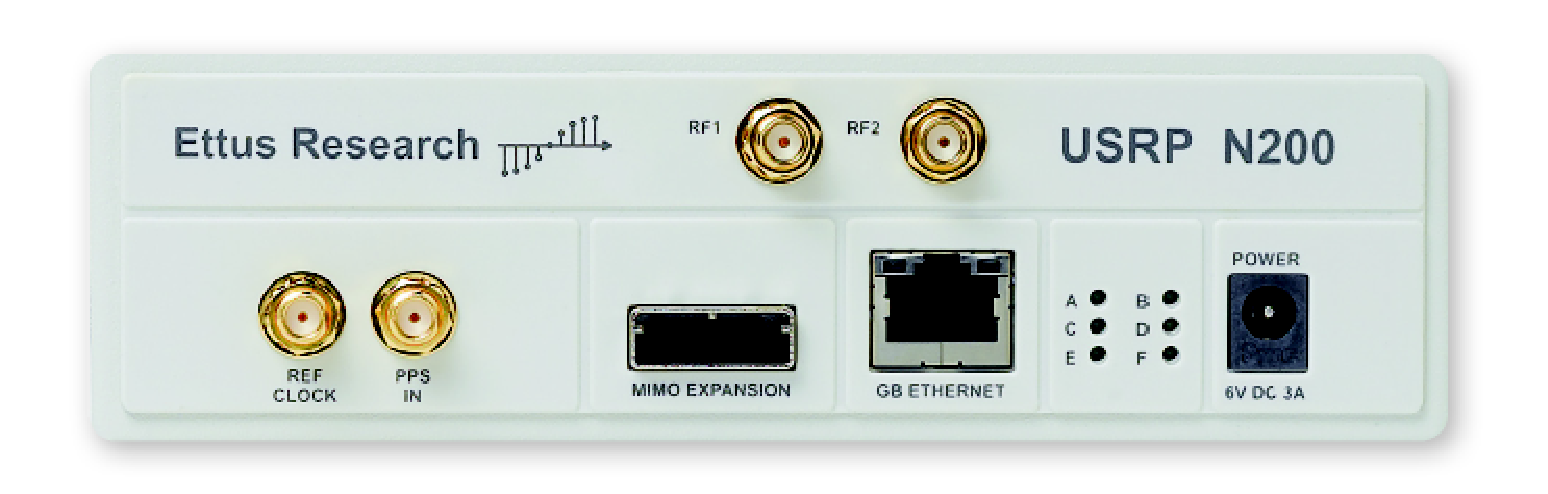
\includegraphics[width=0.65\textwidth]{./figures/usrp}
    \caption{ USRP N210 front view
    \label{fig:usrp}}
\end{figure}

\section{Applications}
\label{sec:sdr_app}

As stated before  at \ref{sdr:overview}, SDR has a wide range of applications,
and very interesting advantages over the current systems. This work shall focus
on the C-RAN and educational applications of \emph{Software Defined Radio}.

\subsection{Military Environment}

The flexibility and adaptability of the Software defined radios have been
getting attention even from the military engineers to be applied in military
radio systems. When it is about military environment, everything has to be as
much reliable as possible, because any fault can cost a human life and having a
good communication system between the troops is a key to be successful in any
incursion.\\

The military environment could benefit a lot from the implementation of SDR
systems, so the Joint Tactical Radio System (JTRS) Program was created by the US
military to develop and produce flexible and interoperable communication
systems, like hand-held communicators, vehicle, airborne and base-stations. The
goal of the JTRS was achieved through SDR systems based on the Software
Communications Architecture (SCA), which uses CORBA on POSIX operating systems
to organize a myriad of software modules.\\

The SCA program provided a flexible, interoperable and scalable system which met
the needs of the military segment through the use of SDR, all the functionality
and expandability is built upon the SCA. The SCA has its military origin but can
and is used by commercial vendors too. The use of SDR outside military and
Network operator environment makes no sense at the first glance, however
software defined radio flexibility can yield substantial benefits in
the longer run, once the fixed costs of implementing it have gone down enough to
overtake the cost of iterated redesign of purpose built systems. This then
explains the increasing commercial interest in the technology.\\

SCA-based infrastructure software and rapid development tools for SDR education
and research are provided by the Open Source SCA Implementation – Embedded
(OSSIE) project. The Wireless Innovation Forum funded the SCA Reference
Implementation project, an open source implementation of the SCA specification.\\

The work in \cite{Chamberlain2005} show an implementation of a Man Pack Radio
using all the SDR techniques, this enlightens the strategic importance of such
systems to the military environment, in incursions or in disaster aid.

\subsection{C-RAN Environment}

C-RAN comes from the cloud idea of Infrastructure as a service (IaaS) or in this
case RAN as a service, thus it needs a reconfigurable and scalable
infrastructure to fulfill the customer needs. SDR is perfect for such
applications because  it is in essence reconfigurable and scalable.\\

The two images below contrast the past RAN infrastructure, still in use today,
with the \emph{Cloud} or \emph{Centralized} RAN for such there is the need of
reconfigurable and scalable front-haul infrastructure. In the C-RAN paradigm all
the processing elements of the systems are centralized in a server-farm like
disposition and the front-haul can be dynamically used depending on the needs of
the network. In the figures \ref{fig:tran} and \ref{fig:cran} it is possible to
observe the evolution from the traditional RAN to the C-RAN paradigm.

%RAN network image
\begin{figure}[htbp]
    \centering
    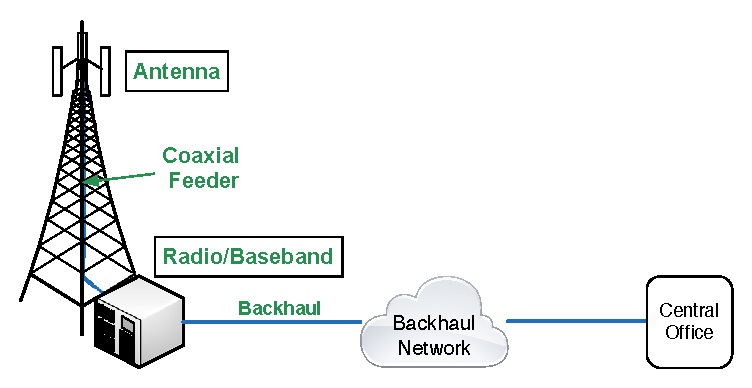
\includegraphics[width=0.65\textwidth]{./figures/traditional_bs}
    \caption{ Traditional Radio Access Netwok
    \label{fig:tran}}
\end{figure}

%C-RAN network image
\begin{figure}[htbp]
    \centering
    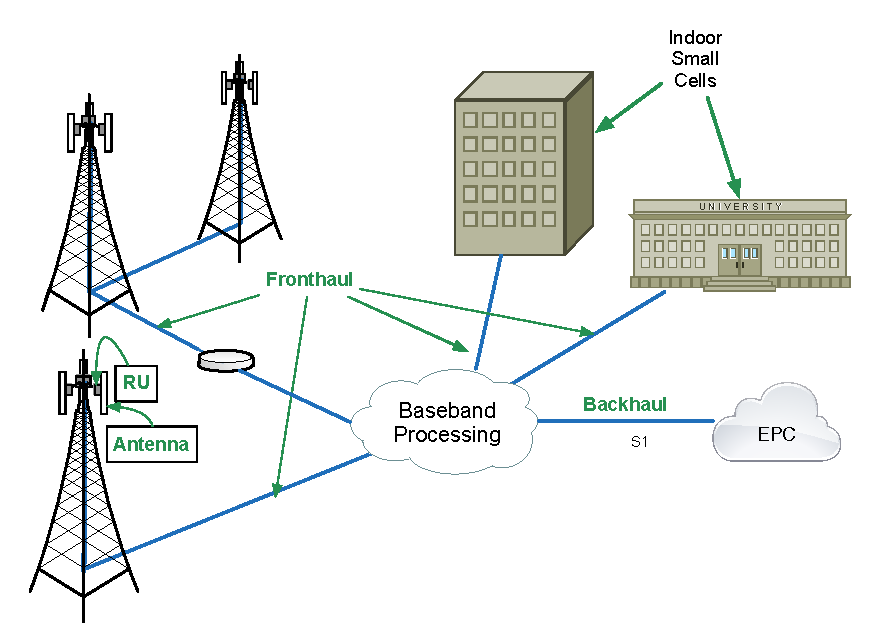
\includegraphics[width=0.65\textwidth]{./figures/c_RAN}
    \caption{ Centralized RAN paradigm.
    \label{fig:cran}}
\end{figure}

There are a lot of works in SDR for modern communication schemes being done in
recent years, and before the concept of CRAN was a buzz they already began to
think how to control SDR in cloud environments \cite{dayananda2012} and other
works were focusing on transmitting on the Ghz frequency band of the modern
communications schemes (3GPP, LTE) \cite{kelley2009} and \cite{neenu2014}.\\

Since the same hardware is used to implement various telecommunications schemes,
the main advantages of the use of SDR in CRAN environment, according to
\cite{dayananda2012} are:

\begin{itemize}
    \item Reduction of costs to maintain Legacy systems;
    \item Reduction of costs and work to upgrade systems;
    \item Easier and cheaper maintenance;
    \item Remote Control over the systems.
    \item Worldwide Roaming made easier.
\end{itemize}


\subsection{Educational Environment}

In the educational environment SDR brings real-world conditions to the lab, the
student or researcher can experiment in a myriad of configurations and make
tests in the real-world channels instead of just simulating a random white
noise, however this is only possible with a hardware implementation of the SDR,
there are still software implementations which use computer sound card ADC and
DAC to communicate on voice range frequencies \cite{ladimer2009}.\\

Having a testbed or simulation to apply all the knowledge acquired in classroom
is crucial to engineering courses, the engineering students often get bored easy
by all the theoretical study and prefer to learn by practice, thus SDR is a
suitable platform to teach digital signal processing, digital communications and
any course related to those subjects.\\

A very famous setup for academic and research in SDR is the duo Gnuradio
\cite{web:gnuradio} and USRP \cite{web:usrp} mentioned in the previous section
\ref{sdr:gnuradio} which can easily implement a communication system with drag
and drop interface\cite{akbook}.\\


\section{Implementations}
\label{sdr:implement}

Software defined radio implementations vary widely depending on available
equipment or type of application, according to \cite{ladimer2009} the basic
architecture of sdr is composed by filters, analog to digital converters (ADC),
digital to analog converters (DAC) and a processor in the core of the system
which could be implemented using DSP for example.\\

\begin{figure}[htbp]
    \centering
    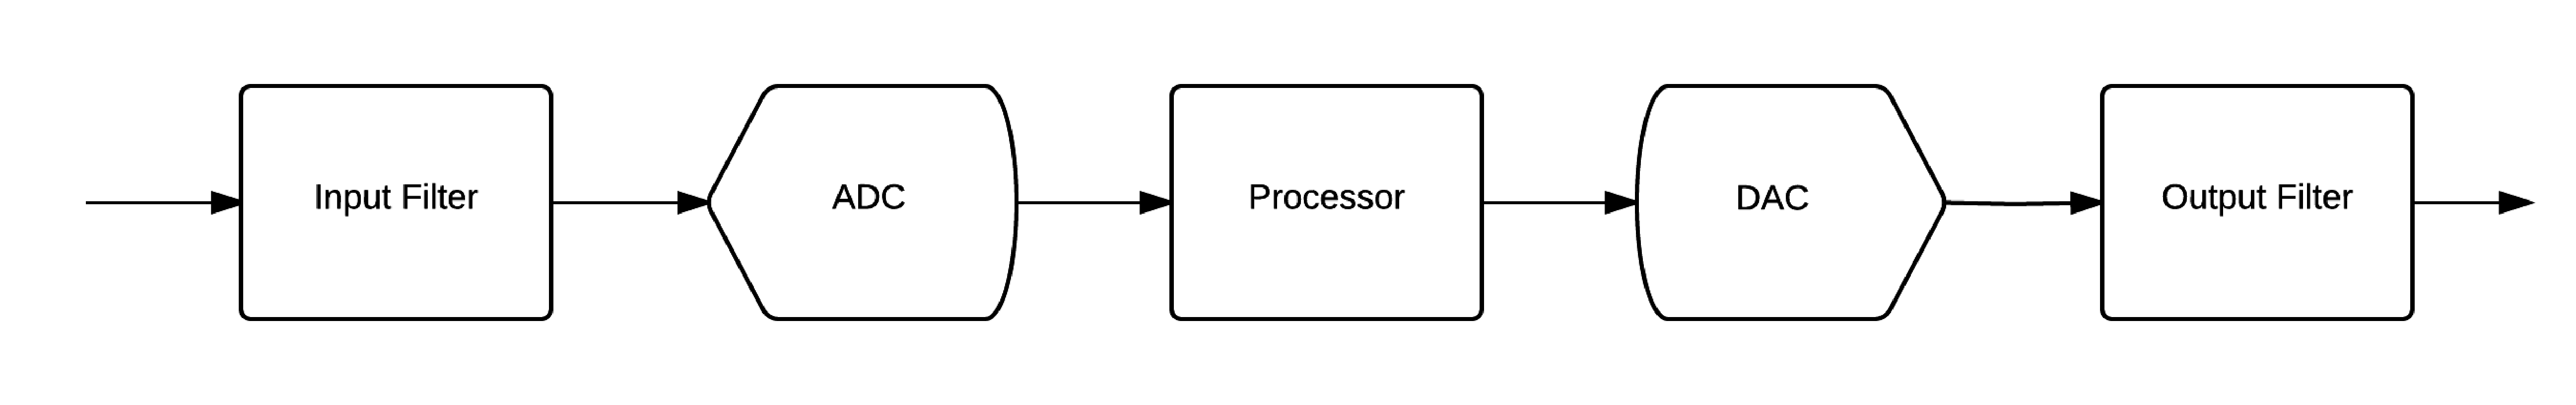
\includegraphics[width=0.8\textwidth]{./figures/sdr_basic_arch}
    \caption{ Software Defined Radio Basic Architecture
    \label{fig:sdr_basic}}
\end{figure}


Implementations may vary a lot, some common implementations are Made in Matlab
through Simulink and use the computer’s sound card as a medium of communication.
A more difficult but more interesting implementation involves the use of DSP
chips to implement the signal processing functions and some cheap ADC and DAC
chips can compose the SDR system.\\

 The most commercial and famous implementation of SDR is Gnuradio+USRP, USRP
stands for Universal Software Radio Peripheral \cite{web:usrp} and Gnuradio
\cite{web:gnuradio}, which was explored in section \ref{sdr:gnuradio}. Gnuradio
plays the role of creating the baseband modulated signals and the passes them
to the USRP to be upconverted and send throught the air. This pair is broadly
used in academic and research environments.\\

When we talk about research and development of real-world systems there is
always a tradeoff or bottleneck, in SDR the bottleneck is the hardware related
to the antenna interface, the antenna is designed to work better in a specific
bandwidth, this can limit the application, of course this is only one example of
bottleneck, there are others like Oscillator frequency, PLL, and processor
capability.\\

This work has a SDR like implementation done in FPGA and using the transceiver
AD9361 which makes baseband upconversion (Transmitter) and downconversion
(Receiver), filters and make analog to digital conversion and digital to analog
conversion, thus it is possible to implement transmitter and receiver with only
one board, however the most complex part does not lie in the system itself
because some electronic parts became a commodity, the complexity is in the
modulation/demodulation blocks and all the synchronization process, such topics
shall be discussed in the chapter \ref{chap:lte}.
